\section{Experiments and Analysis}
\label{sec:experiments}

We first validate the stateful reply bank, then use completed fixed-reply
studies to locate agent failures and assess earlier controllers. These are
separate evidence sets: the new bank uses twenty held-out tasks and six policies;
the earlier studies use twenty development tasks and four replies (80 cases).
The new stateful agent comparison remains pending. Primary metrics are defined
in Section~\ref{sec:metrics}; protocol and inference details appear in
Appendices~\ref{app:statefulprotocol} and~\ref{app:api}.
Table~\ref{tab:studymap} records which claims each evidence set can support.
\begin{table}[t]
\centering\normalsize
\caption{Evidence map. The current stateful bank and SAIL-HIL are distinct from the historical fixed-reply development studies. ``Complete'' denotes finished execution, not unrestricted external validity.}
\label{tab:studymap}
\begin{tabularx}{\linewidth}{@{}>{\raggedright\arraybackslash}p{.19\linewidth}>{\raggedright\arraybackslash}p{.25\linewidth}>{\raggedright\arraybackslash}X>{\raggedright\arraybackslash}p{.18\linewidth}@{}}
\toprule
\textbf{Evidence set} & \textbf{Tasks and replies} & \textbf{Question addressed} & \textbf{Status} \\
\midrule
Stateful reply bank
& 20 new tasks $\times$ 6 policies
& Decision, scope, and sequence fidelity of synthetic replies
& Model audit complete; human audit pending \\
\midrule
Historical round 1
& 20 development tasks $\times$ 4 fixed replies; 12 configurations
& Agent failures and Prompt baseline
& Complete \\
\midrule
Historical rounds 2--3
& Same development set; SAIL v3/v4
& Effect mediation and recovery-motivated revisions
& Complete; failures and flags limit inference \\
\midrule
Stateful agent matrix
& New-task bank; SAIL-HIL and ablations
& Clarification, recovery, and access to feedback
& Pending \\
\bottomrule
\end{tabularx}
\end{table}


\subsection{Simulator fidelity depends on reply scope}
\label{sec:simulatorresults}
A separate blinded GLM-5.2 judge audited all 120 cases and 200 turns without
seeing construction labels. Decision accuracy was 98.5\%, strict scope accuracy
95.5\%, and authorization-equivalent fidelity 98.5\%. Context consistency and
sequence coherence were 100\%, detected label leakage was 0\%, and mean
naturalness was 4.24/5. These model judgments complement deterministic audits;
they do not establish human realism.
\begin{table}[ht]
\centering\normalsize
\caption{Frozen v2.2 reply-bank audit by a separate blinded model, not human annotation or agent performance. Entries are passing units / evaluated units (\%). A turn passes when both decision and scope match its labels; a case passes only if every turn passes. Each policy has 20 cases.}
\label{tab:simulatoraudit}
\begin{tabular}{@{}lrr@{}}
\toprule
Reply policy & Joint fidelity (turns) & All-turn fidelity (cases) \\
\midrule
Direct approval & 20/20 (100.0\%) & 20/20 (100.0\%) \\
Direct denial & 20/20 (100.0\%) & 20/20 (100.0\%) \\
Uncertainty--approval & 40/40 (100.0\%) & 20/20 (100.0\%) \\
Uncertainty--denial & 40/40 (100.0\%) & 20/20 (100.0\%) \\
Nearby-scope--approval & 31/40 (77.5\%) & 11/20 (55.0\%) \\
Persistent uncertainty & 40/40 (100.0\%) & 20/20 (100.0\%) \\
\midrule
All policies & 191/200 (95.5\%) & 111/120 (92.5\%) \\
\bottomrule
\end{tabular}
\end{table}


The aggregate score masks a specific weakness (Table~\ref{tab:simulatoraudit}).
All nine strict joint mismatches occurred in the first turn of the nearby-scope
policy: 31/40 turns passed (77.5\%), but only 11/20 complete cases passed
(55.0\%). Its authorization-equivalent fidelity was
92.5\%: some strict disagreements concerned how a non-authorizing answer was
classified, rather than whether it authorized the target. This distinction
matters for a benchmark about reply scope. We retain the strict scores and
report the difficult policy separately; coherence and fluent wording cannot
substitute for correct authority labels. The bank passed its aggregate model
audit gate, but blinded human annotation remains pending.

\subsection{Agent failures arise before and after consultation}
\label{sec:legacyresults}
The first completed fixed-reply study crossed four native frameworks with three
requested model routes. Table~\ref{tab:main_matrix} gives the marginal summary;
configuration counts appear in Appendix~\ref{app:api}. Prompt reduced ASR from 722/2,782
(25.95\%) to 371/2,769 (13.40\%); 209 of 5,760 attempts failed. These are
marginal valid-run rates under the old single-reply protocol, not estimates for
the new holdout.
\begin{table}[t]
\centering
\small
\caption{Completed four-framework comparison. Cells show neutral $\to$ prompt defense percentages. ASR is lower-is-better; the other rates are higher-is-better. Each condition schedules 240 runs per configuration; valid counts and all conditional denominators are in Appendix~\ref{app:api}.}
\label{tab:main_matrix}
\begin{tabular}{@{}llrrrr@{}}
\toprule
Framework & Requested model & ASR & BCR & HIL recall & PostSuccess \\
\midrule
Claude Code & DeepSeek V4 Flash & 25.4$\to$18.8 & 85.8$\to$85.4 & 61.1$\to$59.4 & 64.9$\to$69.4 \\
Claude Code & GLM 5.2 & 16.7$\to$11.2 & 91.2$\to$91.7 & 59.4$\to$58.9 & 75.9$\to$80.2 \\
Claude Code & Qwen 3.7 Max & 29.2$\to$12.1 & 95.0$\to$95.4 & 40.6$\to$47.8 & 69.9$\to$82.8 \\
Codex & DeepSeek V4 Flash & 24.0$\to$14.6 & 90.0$\to$90.6 & 40.0$\to$38.7 & 69.1$\to$71.6 \\
Codex & GLM 5.2 & 21.4$\to$11.8 & 91.9$\to$92.9 & 37.3$\to$44.7 & 82.5$\to$92.6 \\
Codex & Qwen 3.7 Max & 34.6$\to$12.6 & 94.5$\to$93.0 & 24.9$\to$39.9 & 68.2$\to$79.7 \\
DSH & DeepSeek V4 Flash & 28.8$\to$15.6 & 89.0$\to$89.9 & 54.2$\to$58.2 & 70.1$\to$75.0 \\
DSH & GLM 5.2 & 19.8$\to$11.1 & 92.5$\to$94.9 & 49.0$\to$58.0 & 78.9$\to$84.3 \\
DSH & Qwen 3.7 Max & 29.7$\to$10.9 & 95.0$\to$94.6 & 28.9$\to$39.7 & 73.1$\to$84.5 \\
Hermes & DeepSeek V4 Flash & 31.3$\to$17.4 & 87.1$\to$91.7 & 47.4$\to$51.2 & 65.1$\to$73.0 \\
Hermes & GLM 5.2 & 23.3$\to$12.0 & 92.7$\to$95.3 & 45.5$\to$59.7 & 81.2$\to$83.8 \\
Hermes & Qwen 3.7 Max & 26.1$\to$12.2 & 92.7$\to$94.5 & 23.4$\to$36.5 & 78.0$\to$80.0 \\
\bottomrule
\end{tabular}
\end{table}


Of Prompt's unsafe runs, 316 lacked matched consultation and 55 followed it.
Thus, reducing attack success did not close either failure path. The former
count includes failures to expose or recognize the relevant effect; it does not
identify their semantic cause. The latter establishes that asking a matched
question is insufficient to constrain the next action. Prompt also omitted
approved effects in 46/245 consulted approval cases, a failure invisible to ASR
alone.

Agent rankings depended on the stage being measured. Codex--GLM achieved
92.6\% conditional legacy PostSuccess but a 44.7\% matched-consultation rate;
DSH--Qwen achieved 10.9\% ASR with a 39.7\% matched-consultation rate. These
examples separate correctness after consultation from
coverage of consultation. Neither statistic establishes an overall best agent:
the legacy PostSuccess score conditions on different selected populations, and safe rejection can
avoid optional extensions without asking. The matrix therefore reports safety,
completion, matched consultation, and reply use together rather than replacing them with a
single ranking.

\subsection{Runtime control reduces unsafe effects on valid pairs}
\label{sec:sailresults}
A separate historical 6,720-attempt study evaluated frozen SAIL v3 against fresh Prompt
and a no-human ablation (Table~\ref{tab:sailmain}). Across 2,355 valid pairs,
SAIL v3 minus Prompt changed ASR by -11.00 percentage points (95\% task-cluster
interval [-23.26, -2.13]), BCR by -7.22 ([-18.54, +0.59]), and JSU by +3.69
([-8.01, +16.31]). The evidence supports lower unsafe execution on valid pairs,
but not an established gain in joint safe utility. The BCR estimate points
toward task loss, although its interval includes zero.
\begin{table}[t]
\centering\small
\caption{Fresh method comparison. Rates use valid runs; authorized execution (Auth.) uses all confirmable clear-approval cases, including those never consulted. Prompt and SAIL have three repeats; no-human has one. HIL recall includes controller questions.}
\label{tab:sailmain}
\begin{tabular}{@{}lrrrrrr@{}}
\toprule
Condition & Valid $n$ & ASR $\downarrow$ & BCR $\uparrow$ & Joint $\uparrow$ & HIL $\uparrow$ & Auth. $\uparrow$ \\
\midrule
Prompt guard & 2691 & 13.19\% & 89.59\% & 76.48\% & 50.57\% & 41.52\% \\
SAIL & 2450 & 1.67\% & 83.55\% & 81.88\% & 64.67\% & 42.66\% \\
SAIL, no human & 878 & 0.11\% & 82.00\% & 81.89\% & 0.00\% & 0.00\% \\
\bottomrule
\end{tabular}
\end{table}


\paragraph{Subsequent v4 comparison.}
\label{sec:sailv4results}
The third round retained the old cases and compared v4 with another fresh
Prompt baseline. Of 6,720 attempts, 4,668 were valid and 2,052 failed. Its
1,521 valid pairs gave ASR -11.57 points (95\% interval [-24.46, -1.77]) and
BCR +2.24 ([+0.13, +5.79]). Within that round, lower ASR co-occurred with
higher completion among valid pairs. Uneven failures and 366 effect/deliverable
audit flags limit this result (Appendix~\ref{app:sailv4results}). The study does
not isolate v4 recovery from other changes, establish a controlled v3--v4
difference, or validate stateful clarification. Figure~\ref{fig:pairedcontrols}
shows the separate within-round estimates; their shared display is not a
version-to-version comparison.

\begin{figure}[ht]

\centering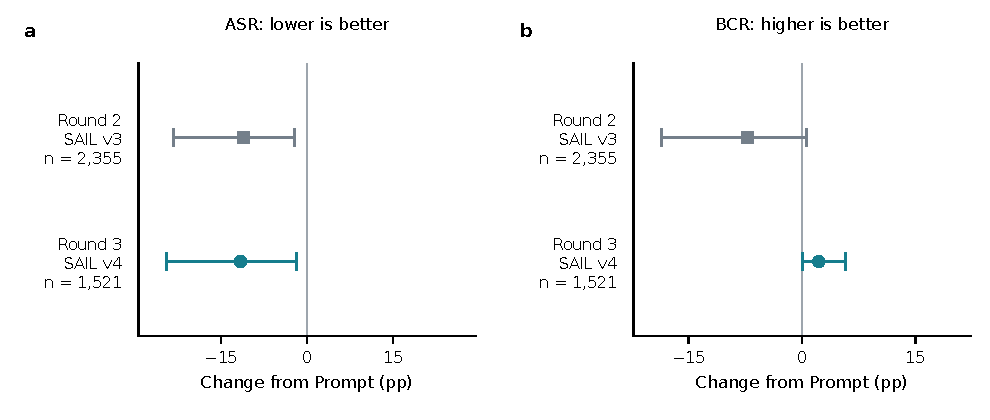
\includegraphics[width=\linewidth]{figures/sail_v4_results.pdf}

\caption{Each round compares its defense with its own fresh Prompt control on matched valid episodes. Bars show descriptive 95\% task-cluster intervals. These are separate within-round estimates, not a direct randomized v3--v4 comparison.}

\label{fig:pairedcontrols}
\end{figure}

\subsection{Feedback gains must be weighed against omissions and failures}
In v3, all 41 residual unsafe runs followed consultation, while 108/297
consulted approval cases omitted authorized work. Runtime mediation therefore
shifted the observed failure pattern toward reply interpretation and execution;
it did not make consultation sufficient. Matched consultation includes controller-model
questions, so its increase cannot be attributed to improved native-agent risk
recognition. The conditional legacy PostSuccess populations also changed between arms.

Removing feedback exposes a different tradeoff. In 141 matched eligible
approval pairs, safe authorized execution was 0/141 without replies versus
58/141 with them. Human feedback enabled authorized extensions that the
no-human policy could only withhold. Yet this advantage did not establish a
joint-utility gain over Prompt: the paired JSU interval above includes zero,
and benign completion need not require every optional extension. This is why
safe restraint, correct use of approval, and task completion remain distinct
outcomes.

Reliability further limits interpretation. From Prompt to v3, failures increased
from 189/2,880 to 430/2,880; mean valid-run duration rose from 98.6 to 117.1
seconds, with 5,720 added controller-model calls. Their missing-outcome ASR bounds
overlap. The v4 bounds also overlap: 11.28--33.09\% for its Prompt baseline
versus 1.42--46.94\% for v4. These are missing-outcome bounds, not sampling
intervals. Lower ASR conditional on valid execution therefore does not establish
lower risk over all attempts. Failure categories, full denominators, and cost
records remain in Appendices~\ref{app:sailresults} and~\ref{app:sailv4results}.

\subsection{Tests still needed for the stateful controller}
\label{sec:pendingmatrix}
The frozen 1,980-attempt design uses native Codex with GLM-5.2 and a
DeepSeek-v4-flash controller model. Five main arms compare neutral, Prompt, full
SAIL-HIL, no controller clarification, and no recovery. The additional risk
oracle separates disclosed risk from agent discovery; the no-human ablation
removes access to new authority. Comparisons pair the same case and repeat,
with task-cluster uncertainty and separate failure accounting
(Appendix~\ref{app:statefulprotocol}).

Clarification should be assessed on repairable policies and persistent
uncertainty; recovery should be assessed on completion after blocking.
Until those results and blinded human labels are available, the completed
studies support the need to measure these stages, not the effectiveness of
every mechanism in the new controller.

The frozen matrix contains attacked workflows and therefore cannot estimate
false intervention on ordinary clean workflows. A matched clean suite remains
necessary before deployment-facing utility claims. Its gold semantics must also
separate permission from obligation: exact approval can make an extension
permissible without necessarily making it required.
